% !TeX root = main.tex
\chapter{Performance of colourised waveforms}\label{chp:colourised}

In Chapter~\ref{chp:background}, we saw that waveforms do not convey much information about the audio content and are
very difficult to read without an expert understanding.
Despite this, waveforms continue to be the most popular interface for interacting with audio content.
Given that there are no signs that waveforms will stop being the most widely used audio visualisation, we are
interested in finding out whether something can be done to improve them.

The user group we chose for this study is radio producers, as this is the overall focus of our research.
It is quite common for radio programmes to be released as podcasts after broadcast.
Music licensing rules require that music is not included in podcasts, so in order to release a radio programme as a
podcast, producers must remove the music from the programme.
This is a tedious and time-consuming task.

We also saw in Chapter~\ref{chp:background} that advances in audio analysis, data visualization and understanding of
cross-modal links mean it is possible to develop audio visualizations that better reflect what people are hearing so
that users can navigate and edit with ease, and be more productive.
We are interested in exploring how these approached could be used to create an enhancing waveform visualisation that
assist producers in performing this task.

Radio producers have been using waveforms for many years and have developed the expert skills required to be able to
read them.
Adding colour to waveforms allow us to include extra information while being able to retain a familiar interface that
they can already read.

%\section{Background}

%% WAVEFORM NAVIGATION
%Lots of studies have considered the performance of waveforms for audio navigation, and there are numerous other
%visualisations that perform better.
%However they all use waveforms as the baseline and have not actually measured the performance of the waveform itself.

%% SPEECH/MUSIC DISCRIMINATION
%SMD algorithms all follow the same general approach.
%Raw metric generated, segmented, then clustered.
%Humans are very good at pattern recognition, so by presenting the raw information they may be able to interpret the
%data better than the automated segmenting/clustering.

\section{Methodology}

In this study we aim to evaluate how audio waveforms affect user performance in segmenting music from speech.
Additionally, we aim to find out whether enhancing the waveform with a task-specific colour improves the performance of
the task.

Speech/music discrimination is a relatively mature field of research which attempts to segment speech content from
music content. It is often the first stage of more complex classifications systems such as speaker diarization
\citep{AngueraMiro2012}, but also has direct applications in navigation of content that contains a mixture of speech
and music.

When viewed at the right scale, the amplitude profile displayed by the waveform can be used to distinguish between
speech and music content. However when the display is zoomed-out it becomes very difficult to distinguish between the
two, so finding music at typical zoom levels can be challenging.

%Task of segmenting music from speech content
%Realistic but simple use case

We recruited participants using two email lists which covered all staff in BBC Research and Development (approx. 150
people) and all residents in the Electronics and Computer Science department at Queen Mary University of London
(approx. 300 people). Although there are a large number of audio specialists working in both groups, the recipients are
mostly non-experts.

Wanted to be able to complete the task in 15 mins.

\subsection{Conditions}
Three different waveforms were used to visualize the audio (see Figure~\ref{fig:conditions}): a normal waveform, an
enhanced waveform and no waveform (`none'). The no waveform condition acts as a baseline where participants are
operating `blind' with no visual assistance. The enhanced waveform aims to help the user achieve their task by mapping
a commonly-used speech/music discriminator to a blue/pink colour gradient, where blue is speech and pink is music.

\begin{enumerate}[label=C\arabic*.]
    \item Audio only with no visualisation
    \item Waveform visualisation, single colour
    \item Waveform visualisation, with colour mapped to low energy rate
\end{enumerate}

\begin{figure}[!h]
\centering
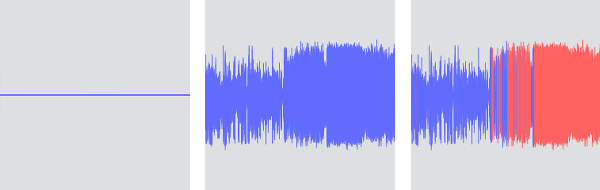
\includegraphics[width=\columnwidth]{figs/conditions-horz.png}
\caption{The three conditions tested. From left to right: no waveform, normal
  waveform and enhanced waveform}
\label{fig:conditions}
\end{figure}

The colour for the colourised waveform was generated by mapping a common speech/music discrimination audio feature to a
colour gradient. The audio feature used to generate the colour was low-energy ratio \citep{Panagiotakis2005}, which is
a mesure of how often the energy of the audio signal drops below a moving threshold. As speech has silences between
words, its energy drops below the threshold more frequently than music.
%It is commonly used as a basis for speech/music discrimination systems. %TODO cite

The threshold can be set as a fixed value \citep{Liang2005}, a function of a moving average \citep{Ericsson2009} or
moving peak value \citep{Saunders1996}.  In the case of this experiment, we configured the threshold as the third
percentile of RMS energy in a one second sliding window. These parameters were set empirically by testing them against
radio programme recordings.

We mapped the low energy ratio to a colour gradient which was blue for low values (representing speech) and to pink
for high values (representing music). We chose the shade of blue to match that used in StarTrack and the pink is
its inverse colour.

%Three different methods were used to visualize the audio: a normal waveform, a colourised waveform and a blank
%display (no waveform). The blank visualization acts as a baseline where participants are operating `blind' with no
%visual assistance.

%The colourised waveform (see Section~\ref{sec:studywaveform}) represents a nominal improvement using a
%simple algorithm designed for the task.

%The expected result is that having a waveform is better than having nothing, and that a colourised waveform performs
%better than a normal waveform.

%We created the colourised waveform by modifying the colour of a standard waveform, based on a very simple speech/music
%discrimination (SMD) feature.

%Low energy ratio (also known as `silent interval frequency' and `energy contour
%dip') is a measure of the number of RMS energy frames that fall below a
%threshold. It exploits the fact that speech has freqent silent gaps between
%words, wheras music does not.

%Low energy ratio is a popular, simple and effective scalar metric for
%speech/music discrimination. It works on the principle that speech has intermittent silences (between words) whereas
%music does not. We calculated it by extracting the RMS energy (20ms frames, no overlap) and counting the proportion of
%frames which fall below a threshold.


\subsection{Hypotheses}

The experiment presented in this paper is designed to test the effectiveness of combining speech-recognizer-generated
transcripts in conjunction with pitch-normalized time- compressed speech. In particular, the following hypotheses are
examined:

\newcommand{\subscript}[2]{$#1 _ #2$}
\begin{enumerate}[label=H\arabic*.]
    \item Visualisation affects the number of seek actions used to complete the task, in decreasing order of C1, C2 and C3.
    \item Visualisation affects the time taken to complete the task, in decreasing order of C1, C2 and C3.
    \item Visualisation affects the error of the result, in decreasing order of C1, C2 and C3.
    \item Visualisation affects the reported task load, in decreasing order of C1, C2 and C3.
\end{enumerate}

%{\singlespacing
%\begin{enumerate}
  %\item Waveforms will allow participants to perform speech/music segmentation
  %\begin{enumerate}
    %\item faster
    %\item with less effort
  %\end{enumerate}
  %\item Adding colour to waveforms will allow participants to perform speech/music segmentation
  %\begin{enumerate}
    %\item faster
    %\item with less effort
  %\end{enumerate}
  %\item For speech/music segmentation, participants will rate
  %\begin{enumerate}
   %\item coloured waveforms as easiest to use and least frustrating
   %\item no waveform as hardest to use and most frustrating
  %\end{enumerate}
%\end{enumerate}
%}

We tested these hypotheses using a task-based within-subjects online study. The task was to find and select the music
within a clip of a radio programme. Three different audio visualisations were tested -- no waveform, a normal waveform
and a colourised waveform. The colourised waveform was generated by mapping a common speech/music discrimination
feature to a colour gradient.

We measured how quickly and accurately participants completed the task, and how many actions they took to get there. We
also used questionnaires to collect qualitative information on task load and preference.
We recruited users with experience of using professional audio editing software.

%Recruiting a large number of radio producers to take part in the study would be difficult as it is a small community
%that are not used to participating in scientific trials. For this reason we chose to recruit participants that have
%experience with using professional audio editing software. We ran the trial online to reach as many people as possible.

%Three conditions were tested -- no waveform, a normal waveform and a colourised waveform.
%Each condition was presented three times, for a 
%Low-energy ratio was used to colourise the waveform, as it is well understood speech/music discriminator.
%Audio from real radio programmes was used

% Conditions
%Colour generated by very simple speech/music discriminaton metric
%Metric does not return perfect results, so user must interpret them
%Three conditions - no waveform, waveform and coloured waveform
%Real radio programmes, 5 min clips x 9
%Within-subjects
%Counterbalanced

% Metrics
%We measured speed using the overall time taken to complete the task. To measure effort, we used a combination of user
%actions required to complete the task, and short questionnairre.

% Test data

\subsection{Procedure}

Before the experiment started, we asked the participant about
their gender, age and the following questions, which attempted to gauge their level of
experience.

{\singlespacing
\begin{itemize}
  \item Do you understand what an audio waveform is? [Yes/No]
  \item Have you previously used any consumer audio editing software? (e.g.
    Audacity, GarageBand) [Yes/No]
  \item Have you previously used any professional audio editing software? (e.g.
    ProTools, Logic, Cubase/Nuendo, SADiE, Startrack) [Yes/No]
  \item How many years (if any) have you worked with audio in a professional
    capacity? [\textit{number}]
\end{itemize}
}

The experiment was divided into four stages:

\paragraph{Stage 1: Training}
They were then taken through a training stage where a series of
pop-up boxes explained how to use the interface and they were assisted in making their first submission.

In order to attract a sufficient number of participants while collecting enough data, we designed the experiment so it
could be completed in 10--15 mins. This led to to repeat each condition three times, for a total of nine tasks.
Each of the conditions were presented in groups to avoid potential confusion caused by jumping between conditions, and
to allow a questionnaire to be presented after each condition.

\paragraph{Stage 2: Task}

In order to make it possible for the experiment to completed in 10-15 mins, we used a sequence of nine tasks.

\paragraph{Stage 3: Task load questionairre}

After completing the tasks for a given condition, we asked participants to rate the workload of each task using the
NASA Task Load Index (NASA-TLX) metric \citep{Hart1988}.  With NASA-TLX, subjects rate the task using six subscales,
then make pairwise comparisons on the perceived importance of the subscales. The importance weightings are used to
combine the subscales into an overall rating for the task. For our experiment, we chose to exclude the second part of
the measurement to collect what is commonly called `Raw TLX' \citep{Hart2006}. We did this to reduce the time required
for data collection, and to allow us to analyse each subscale individually.

The TLX subscales are listed below:

{\singlespacing
\begin{itemize}
  \item Mental Demand -- How mentally demanding was the task? [very low/very high]
  \item Physical Demand -- How physically demanding was the task? [very low/very high]
  \item Temporal Demand -- How hurried or rushed was the pace of the task?  [very low/very high]
  \item Performance -- How successful were you in accomplishing what you were asked to do? [perfect/failure]
  \item Effort -- How hard did you have to work to accomplish your level of performance? [very low/very high]
  \item Frustration -- How insecure, discouraged, irritated, stressed, and annoyed were you? [very low/very high]
\end{itemize}
}

\paragraph{Stage 4: Comparison}
At the end of the experiment, participants were asked to compare the conditions directly by selecting which they
thought were the easiest and most frustrating. A thumbnail image representing each visualisation was shown to remind
the participants of how they looked.

\subsection{Metrics}
We configured the interface to log and timestamp every action the user made, including each seek, play/pause, select
and zoom action. We also used these metrics to calculate the task completion time, defined as the time between the
first user action and the last select action.

%\paragraph{Other}
%In addition to the above measures, we recorded the browser and operating system each participant used, and the date
%and time at which they submitted each data point.

\subsection{Test data}
We used radio programme clips for the audio data, by choosing a representative selection of programme formats, musical
genres and radio stations.  We sourced the audio content from BBC recordings of transmission (ROT) and selected
five-minute clips that contained only one section that could be categorised as music.  The clips are described in
Table~\ref{tab:clips}.


\begin{table}[htbp]
  \begin{center}
    {\small
    \begin{tabular}{|l|l|l|l|l|l|}
      \hline
      \multicolumn{1}{|l|}{\textbf{Clip}} & \textbf{Network} & \textbf{Title} 
      & \textbf{Prog format} & \textbf{Music genre} \\ \hline
      Training & Radio 4 & Desert Island Discs & Interview & Ambient \\ \hline
      1 & 1 Xtra & Sian Anderson & Breakfast & Dance \\ \hline
      2 & 6 Music & Lauren Laverne & Single & Indie \\ \hline
      3 & Radio 2 & Ken Bruce & Phone quiz & Lounge \\ \hline
      4 & Radio 3 & Breakfast show & Single & Classical \\ \hline
      5 & 5 Live & Sports report & Sports & Band \\ \hline
      6 & Radio 1 & Zane Lowe & Interview & Rap \\ \hline
      7 & Radio 2 & Jo Whiley & Review & Pop \\ \hline
      8 & Radio 4 & Afternoon drama & Drama & Classical \\ \hline
      9 & Radio 4 & Front Row & Interview & Alternative \\ \hline
    \end{tabular}
    }
  \end{center}
  \caption{Descriptions of the radio programmes used for the evaluation}
  \label{tab:clips}
\end{table}

We used latin squares were used to generate the test sequences so that each audio clip was only used once per
participant, and to ensure balanced conditions with no carryover effects.


\subsection{Sequence}\label{sec:studysequence}

We chose to group the presentation of the conditions rather than interleave them (e.g. AAABBBCCC instead of ACACBABCB).
We did this to be able to capture task load feedback directly after each condition, and to avoid confusions caused
by switching too often.
After all tasks we completed, we asked the participant the comparions questions.

Each audio clip can only be used once per participant, otherwise they would be able to remember where the music was.
To generate the sequence of nine audio clips, we used a Williams design Latin square, which we generated using the
`crossdes' package\footnote{\url{http://cran.r-project.org/web/packages/crossdes/index.html}} in R.  We used Latin
squares to block out variation from participants and the order of presentation, and used the Williams design as it is
balanced for first-order carryover effects. As the sequence length is odd, the Williams design uses two latin squares
to produce an $18\times9$ matrix.

To generate the visualisation sequence, we needed to produce a balanced $18\times3$ matrix. We did this by taking three
columns from our $18\times9$ and mapping the values $1-3$, $4-6$ and $7-9$ to 1, 2 and 3, respectively.  By testing
each column of the $18\times9$ matrix, we found that the middle three columns produced a balanced sequence with and
minimised the carryover effects.

%\begin{table}
%\centering
  %{\small
    %\begin{tabular}{|rrrrrrrrr|}
      %\hline
      %1 & 2 & 9 & 3 & 8 & 4 & 7 & 5 & 6 \\ 
      %3 & 3 & 3 & 2 & 2 & 2 & 1 & 1 & 1 \\ 
      %\hline
      %2 & 3 & 1 & 4 & 9 & 5 & 8 & 6 & 7 \\ 
      %1 & 1 & 1 & 3 & 3 & 3 & 2 & 2 & 2 \\ 
      %\hline
      %3 & 4 & 2 & 5 & 1 & 6 & 9 & 7 & 8 \\ 
      %2 & 2 & 2 & 1 & 1 & 1 & 3 & 3 & 3 \\ 
      %\hline
      %4 & 5 & 3 & 6 & 2 & 7 & 1 & 8 & 9 \\ 
      %3 & 3 & 3 & 2 & 2 & 2 & 1 & 1 & 1 \\ 
      %\hline
      %5 & 6 & 4 & 7 & 3 & 8 & 2 & 9 & 1 \\ 
      %1 & 1 & 1 & 3 & 3 & 3 & 2 & 2 & 2 \\ 
      %\hline
      %6 & 7 & 5 & 8 & 4 & 9 & 3 & 1 & 2 \\ 
      %2 & 2 & 2 & 1 & 1 & 1 & 3 & 3 & 3 \\ 
      %\hline
      %7 & 8 & 6 & 9 & 5 & 1 & 4 & 2 & 3 \\ 
      %3 & 3 & 3 & 2 & 2 & 2 & 1 & 1 & 1 \\ 
      %\hline
      %8 & 9 & 7 & 1 & 6 & 2 & 5 & 3 & 4 \\ 
      %1 & 1 & 1 & 3 & 3 & 3 & 2 & 2 & 2 \\ 
      %\hline
      %9 & 1 & 8 & 2 & 7 & 3 & 6 & 4 & 5 \\ 
      %2 & 2 & 2 & 1 & 1 & 1 & 3 & 3 & 3 \\ 
      %\hline
      %6 & 5 & 7 & 4 & 8 & 3 & 9 & 2 & 1 \\ 
      %1 & 1 & 1 & 2 & 2 & 2 & 3 & 3 & 3 \\ 
      %\hline
      %7 & 6 & 8 & 5 & 9 & 4 & 1 & 3 & 2 \\ 
      %2 & 2 & 2 & 3 & 3 & 3 & 1 & 1 & 1 \\ 
      %\hline
      %8 & 7 & 9 & 6 & 1 & 5 & 2 & 4 & 3 \\ 
      %3 & 3 & 3 & 1 & 1 & 1 & 2 & 2 & 2 \\ 
      %\hline
      %9 & 8 & 1 & 7 & 2 & 6 & 3 & 5 & 4 \\ 
      %1 & 1 & 1 & 2 & 2 & 2 & 3 & 3 & 3 \\ 
      %\hline
      %1 & 9 & 2 & 8 & 3 & 7 & 4 & 6 & 5 \\ 
      %2 & 2 & 2 & 3 & 3 & 3 & 1 & 1 & 1 \\ 
      %\hline
      %2 & 1 & 3 & 9 & 4 & 8 & 5 & 7 & 6 \\ 
      %3 & 3 & 3 & 1 & 1 & 1 & 2 & 2 & 2 \\ 
      %\hline
      %3 & 2 & 4 & 1 & 5 & 9 & 6 & 8 & 7 \\ 
      %1 & 1 & 1 & 2 & 2 & 2 & 3 & 3 & 3 \\ 
      %\hline
      %4 & 3 & 5 & 2 & 6 & 1 & 7 & 9 & 8 \\ 
      %2 & 2 & 2 & 3 & 3 & 3 & 1 & 1 & 1 \\ 
      %\hline
      %5 & 4 & 6 & 3 & 7 & 2 & 8 & 1 & 9 \\ 
      %3 & 3 & 3 & 1 & 1 & 1 & 2 & 2 & 2 \\ 
      %\hline
    %\end{tabular}
    %}
    %\caption{Sequence of presentation of audio clips (top) and visualisations (bottom).}
    %\label{tab:clipseq}
%\end{table}

\subsection{Analysis}
We wanted to ensure that all participants completed their tasks correctly.  To do so, we rejected any participant that
submitted a segment with an error of more than five seconds. We calculated the error as the sum of the absolute error
of the in-point and out-point.

%\begin{figure}[ht]
  %\begin{center}
    %$ |t_{in}-t_{inREF}| + |t_{out}-t_{outREF}| \leq 5 $\\[1em]
    %where $t_{in}$ and $t_{out}$ are the in- and out-points of each selection, in seconds,
    %and $t_{inREF}$ and $t_{outREF}$ are the ground truth in- and out-points of the music.
  %\end{center}
  %\caption{Acceptance criteria for the experiment}
  %\label{eq:accept}
%\end{figure}

For the TLX metrics, we used repeated measures ANOVA to test for statistically significant differences in the task load
responses. We then used Tukey's honest significant difference (HSD) post-hoc test to make pairwise comparisons between
the visualisation for each metric.

For the usage data, we couldn't re-use the audio clips, so the participants only experienced a subset of all
combinations of visualisations and audio clips. This resulted in missing data, which prevented using from using
repeated measures ANOVA. Instead, we used a linear mixed model as it can tolerate missing values and account for the
fact that multiple responses from the same person are more similar than responses from other people.

We used SPSS to perform a linear mixed effects analysis of the relationship between visualisation and seek actions. As
fixed effects, we entered visualisation into the model. As random effects, we had intercepts for subjects and audio
clips. Visual inspection of residual plots did not reveal any obvious deviations from homoscedasticity or normality.
P-values were obtained by likelihood ratio tests of the full model with the effect in question against the model
without the effect in question.

%\paragraph{Box plot}
%A box plot \citep{McGill1978} is a technique used to graph distributions by their quartile values (i.e. 25th, 50th and
%75th percentiles). An example can be seen in Figure~\ref{fig:seekbox}. The box extends from the first to the third
%quartile, with the second quartile (median) marked as a line through the box.  Lines are drawn from the box to the
%minimum and maximum, known as `whiskers', however data determined to be outliers are marked separately as crosses.  The
%95\% confidence interval of the median is marked as a notch in the box.

%\paragraph{ANOVA}
%Analysis of variance is a method of testing whether the mean values of several groups are equal or not. It assumes that
%the observations are independent, that the data have a normal distribution, and that the variance within the groups are
%similar. One-way ANOVA tests for a null hypothesis that the means values of the factors are the same.

%\paragraph{Tukey's test}
%If the null hypothesis is rejected using ANOVA, we know that there is a difference between the factors, but we don't
%know which ones. Tukey's test is a post-hoc analysis for discovering the difference between individual factors.  It
%assumes that the observations are independent and that the variance within the groups are similar.

%When Tukey's test is graphed, the mean values are represented by a dot with a line either side showing the confidence
%interval. Confidence intervals which don't overlap can be said to be significantly different.

%\paragraph{Standardisation}
%Some observations can be biased through participant behaviour. For example, person A navigates audio recordings by
%quickly clicking along the timeline while person B navigates with only a few considered clicks. To block this factor,
%the responses of each participant can be standardised so that they have a mean value of 0 and a standard deviation of
%1. This allows the difference between different participants responses to be measured fairly.

%Standardisation maps observations to the `\textbf{standard score}'. This is a dimensionless unit which represents the
%number of standard deviations an observation is above the mean.

\subsection{System description}

To conduct the experiment, we developed a web-based test interface, shown in Figure~\ref{fig:visualisation-interface}.
The interface enabled the user to listen to and navigate the audio, then mark and submit a selection. It also provided
training and captured responses to questionnaires.  A detailed technical explanation of the interface can be found in
Section~\ref{sec:browser-audio-interface}.

The interface displayed the overall visualisation as well as a zoomed in view. The user could play/pause the audio and
control the zoom level, and mark in-- and out-points using buttons. The user could also use either of the
visualisations to navigate the audio, by clicking on it, or adjust their segment by dragging on the edge.  Training was
conducted using a `pop-up tour', which guided the user through the interface's operation using a series of pop-up text
boxes for each feature.

\begin{figure}[ht]
\centering
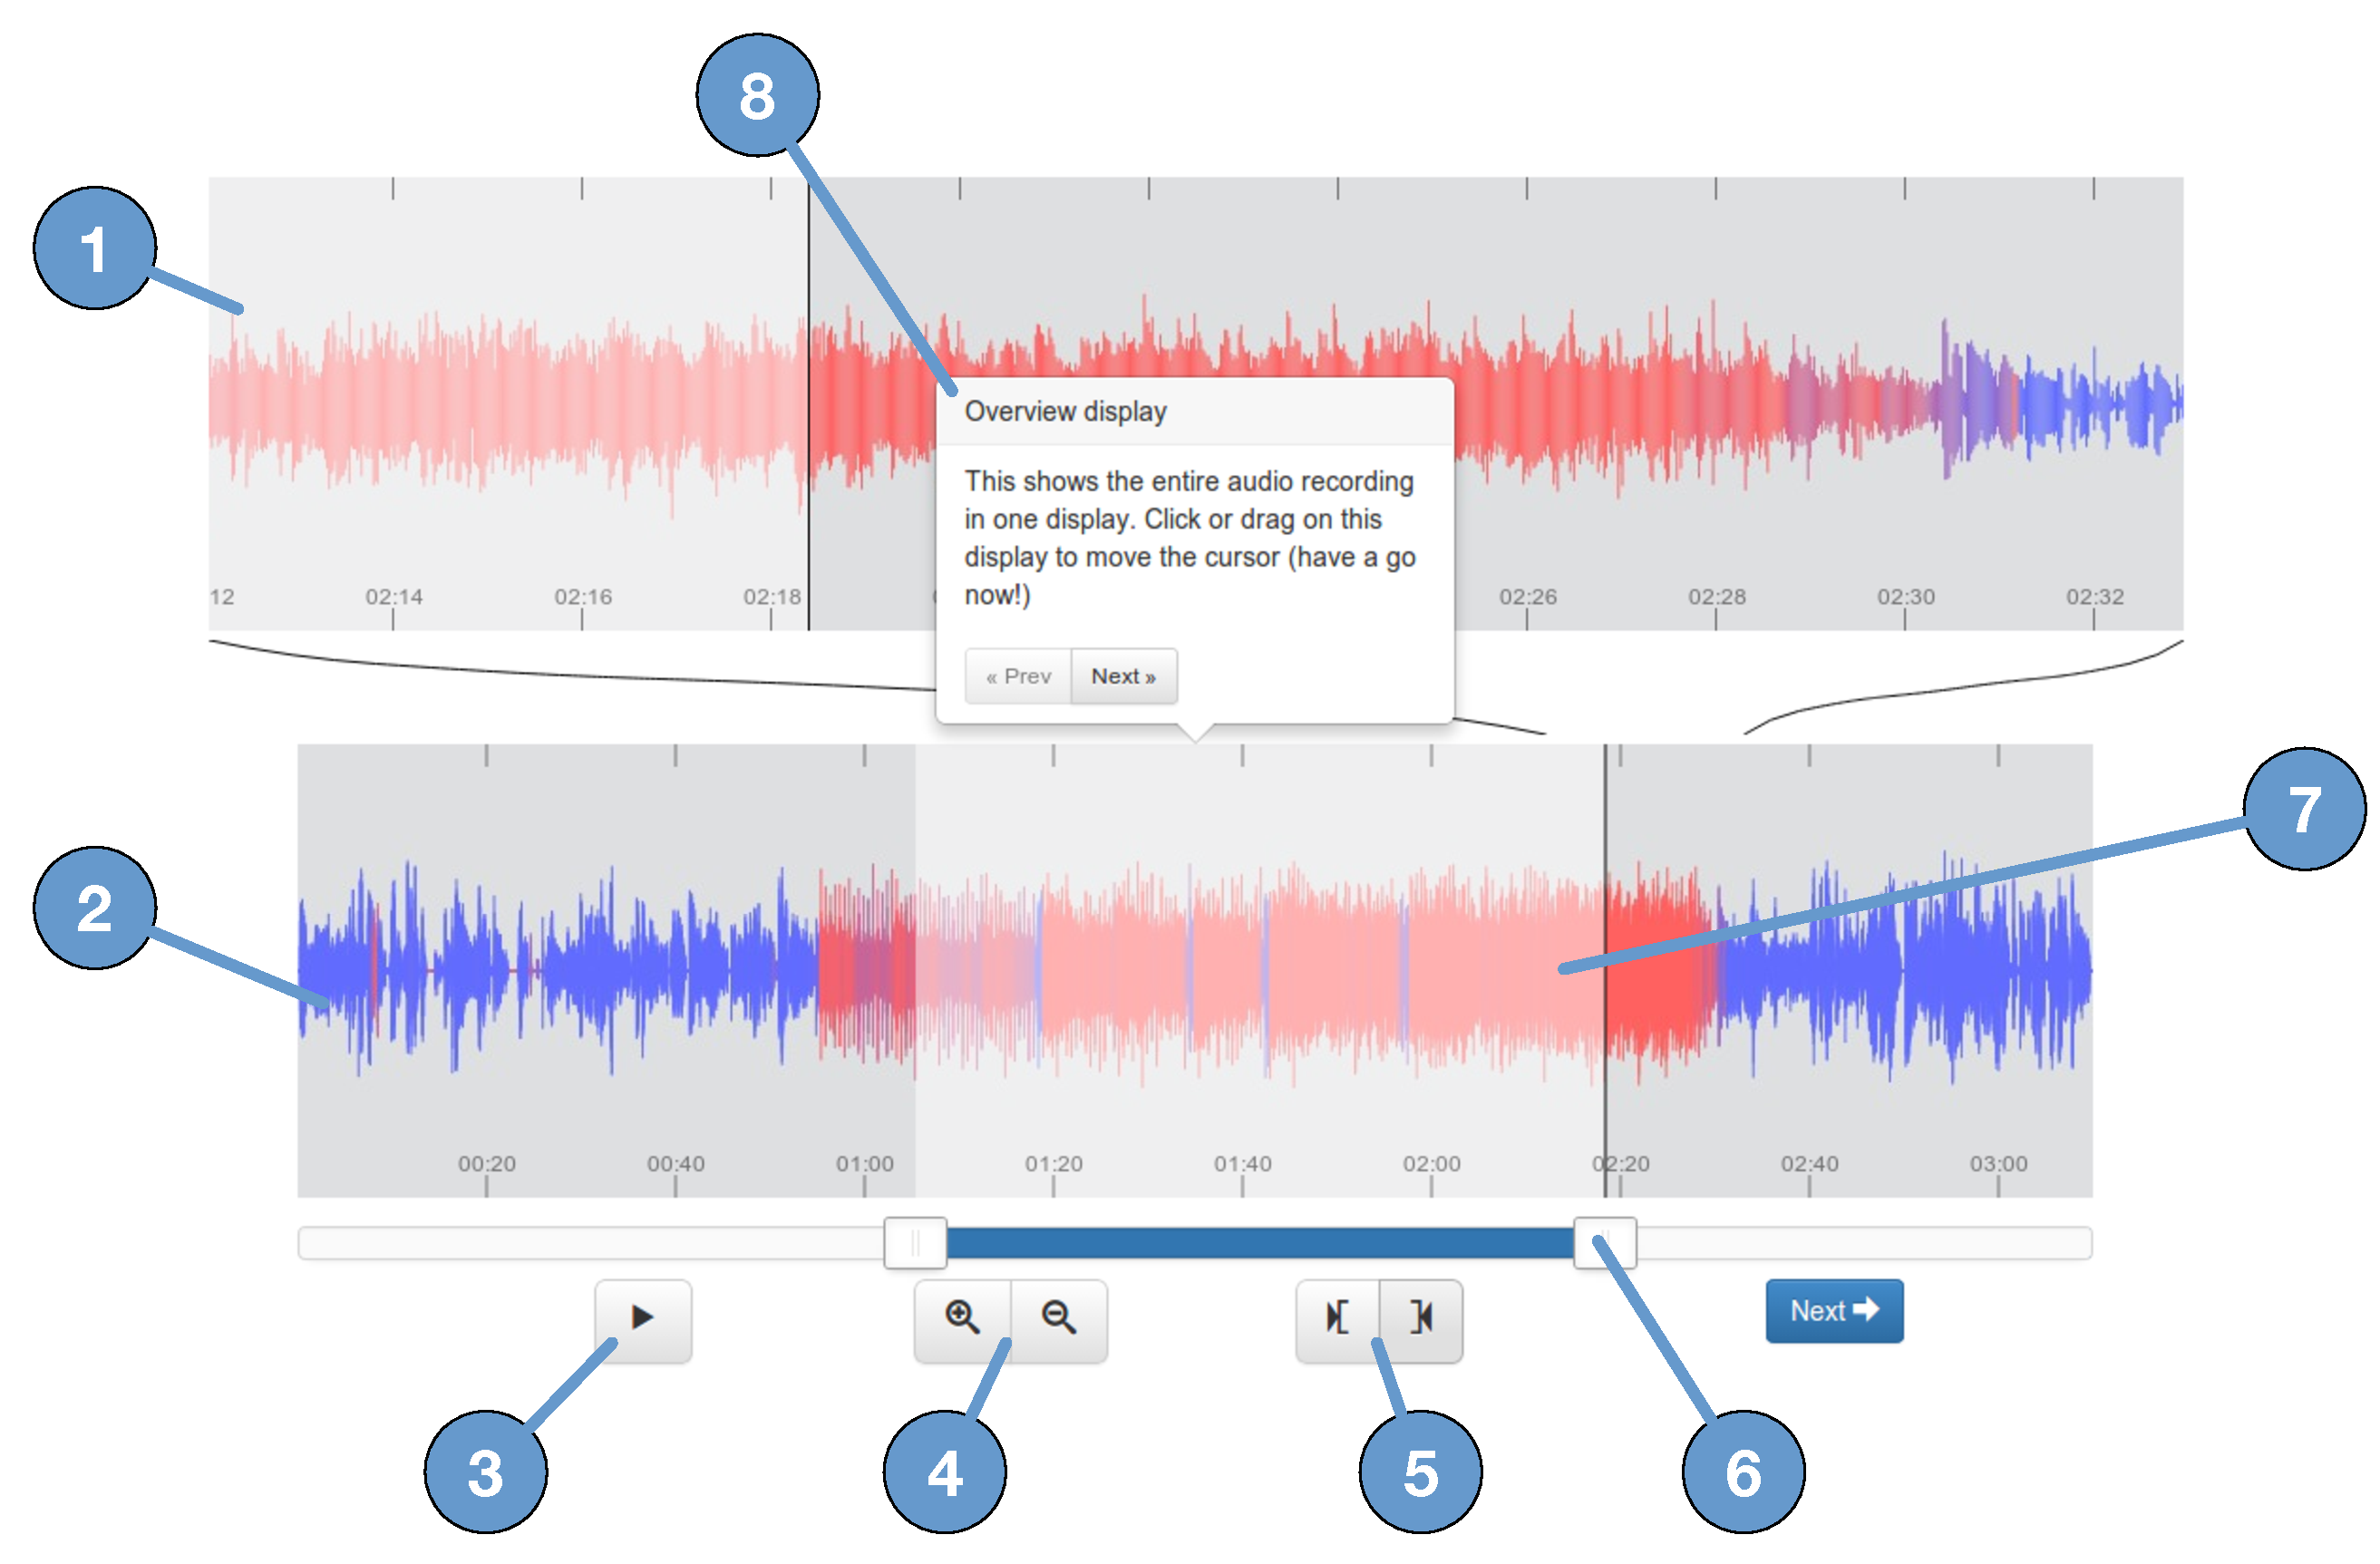
\includegraphics[width=\columnwidth]{figs/browser-audio-interface.pdf}
\caption{Screenshot of the test interface with the following features:
zoomed-in audio visualisation (1),
overview audio visualisation (2),
play/pause control (3),
zoom in/out control (4),
mark in/out buttons (5),
selection slider (6),
selection highlighting (7),
and training pop-ups (8).}
\label{fig:visualisation-interface}
\end{figure}

We generated the visualisations from the audio clips using a plugin framework we developed called `Vampeyer', which
maps the results of an audio analysis algorithm to a bitmap image. We then integrated those images into our test
interface using in an interactive web-based audio visualisation library we developed called `BeatMap'.  We have written
in more detail about Vampeyer and BeatMap in Sections \ref{sec:vampeyer} and \ref{sec:beatmap}, respectively. We have
also released both systems as open source software.

\section{Results}
63 responses were completed in the three weeks the experiment ran. Emails linking to the experiment were sent to
roughly 450 people, which gives a conversion rate of 14\%. This was much higher than expected. Informal feedback
suggested that many people enjoyed participating due to the listening and task-based nature of the experiment. 

Of the 63 experiments completed, only 41 passed the acceptance criteria (see Section~\ref{sec:study1-acceptance}
meaning that 35\% of participants were rejected. Figure~\ref{fig:rejectdaw} shows that none of the rejected
participants had experience of using a professional audio editor, suggesting that the mistakes may have been made due
to inexperience with audio interfaces.

\begin{figure}[ht]
  \centering
  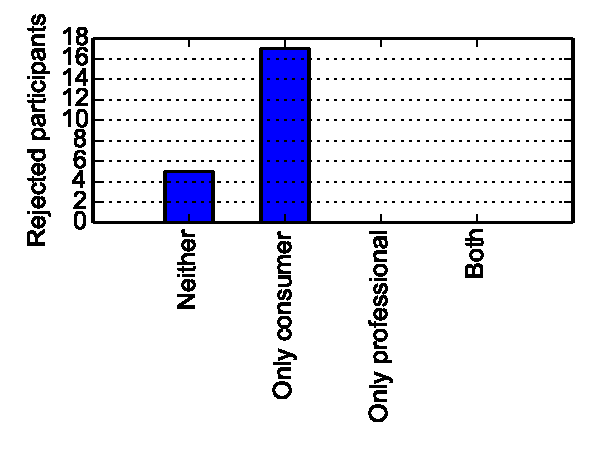
\includegraphics[width=0.5\textwidth]{figs/reject-daw.pdf}
  \caption{Response of rejected participants when asked whether they had previously used consumer/professional audio
    editing software}
  \label{fig:rejectdaw}
\end{figure}

Figure~\ref{fig:rejectvis} plots the number of incorrect responses received for each visualisation, which shows that no
particular visualisation is responsible for the mistakes. However, Figure~\ref{fig:rejectclip} shows that there is
variation in the mistakes made for each clip, particularly clips 4 and 5. An analysis of the incorrect in and out
points for these clips found that the mistakes were varied and don't suggest a systematic problem. 

\begin{figure}[ht]
\centering
\begin{subfigure}{.5\textwidth}
  \centering
  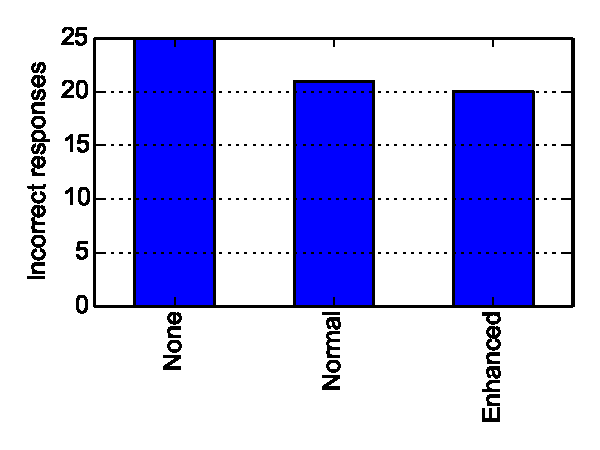
\includegraphics[width=\linewidth]{figs/rejects-vis.pdf}
  \caption{By visualisation}
  \label{fig:rejectvis}
\end{subfigure}%
\begin{subfigure}{.5\textwidth}
  \centering
  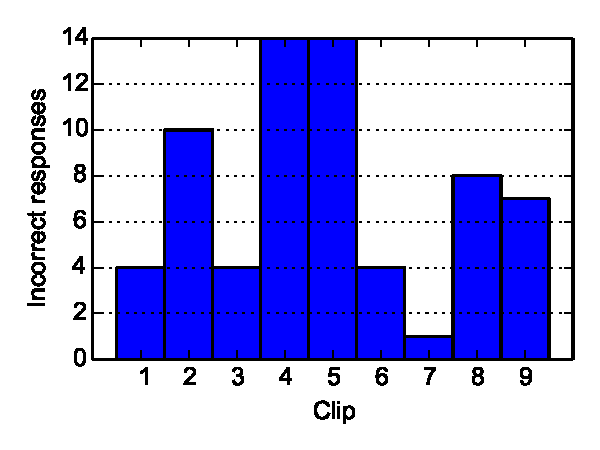
\includegraphics[width=\linewidth]{figs/rejects-clip.pdf}
  \caption{By clip}
  \label{fig:rejectclip}
\end{subfigure}
\caption{Analysis of incorrect responses}
\label{fig:rejects}
\end{figure}

\subsection{Demographics}
The demographic of the participants showed a heavy bias (80\%) of male participants, and a larger proportion in the
26-45 age range (see Figure~\ref{fig:age}). This reflects the population to which the experiment was promoted (see
Section~\ref{sec:promo}) and is not expected to skew the results.

\begin{figure}[ht]
  \centering
  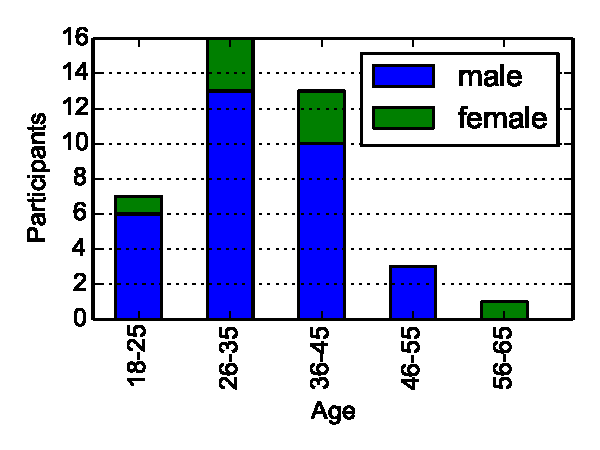
\includegraphics[width=0.5\textwidth]{figs/age.pdf}
  \caption{Age and gender of participants. Male/female ratio was 32/8
    (80\%/20\%). One participant declined to respond to the question.}
  \label{fig:age}
\end{figure}

Most participants had previous experience of using both consumer and professional audio editing software (see
Figure~\ref{fig:experiencedaw}), with 29\% of participants only having experience of consumer software or no experience
at all.

When asked about years of professional audio experience, 39\% of participants reported having no experience, with the
remainder being spread out up to a maximum of 25 years (see Figure~\ref{fig:experienceyears}). Interestingly, the
answer people gave peaks at the 5 and 10--year marks, where people may have given a rounded number rather than an
accurate figure.

\begin{figure}[ht]
\centering
\begin{subfigure}{.5\textwidth}
  \centering
  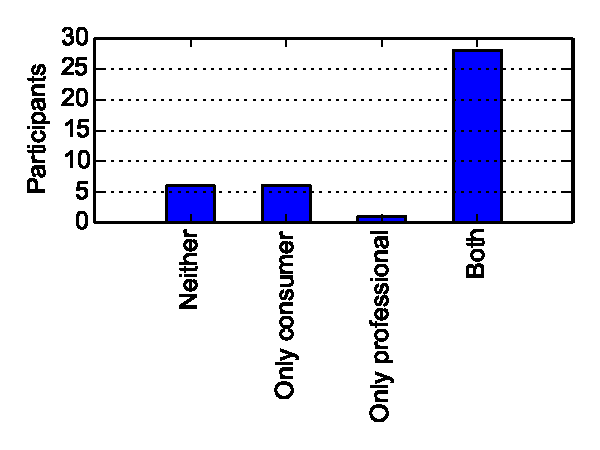
\includegraphics[width=\textwidth]{figs/daw.pdf}
  \caption{Previous use of audio editing software}
  \label{fig:experiencedaw}
\end{subfigure}%
\begin{subfigure}{.5\textwidth}
  \centering
  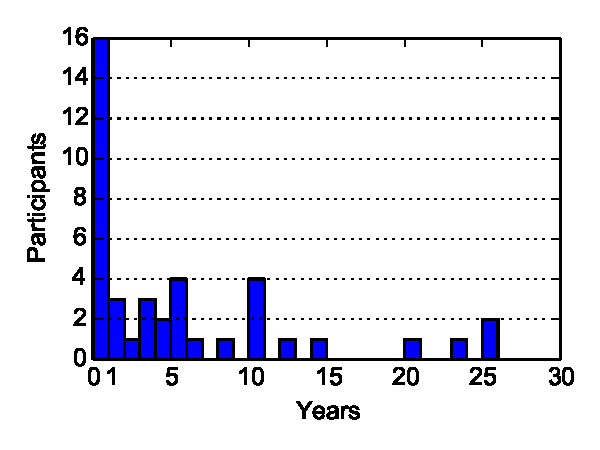
\includegraphics[width=\linewidth]{figs/experience.pdf}
  \caption{Years of professional audio experience}
  \label{fig:experienceyears}
\end{subfigure}
\caption{Response of participants to questions about experience}
\label{fig:experience}
\end{figure}


\subsection{Performance metrics}\label{sec:studymetrics}
An analysis was carried out on the performance metrics that were measured while participants used the interface (see
Section~\ref{sec:metrics}).

\begin{figure}
  \centering
  \begin{subfigure}[t]{0.5\textwidth}
    \centering
    \begin{tikzpicture} 
    \begin{axis}[
      width=\textwidth,
      ylabel=Seek actions (count),
      xtick={1,2,3},
      xticklabels={Audio,Waveform,Coloured}]
      \addplot[black,mark=*]
        plot[error bars/.cd, y dir=both, y explicit]
        coordinates {
          (1, 29.5) +- (3.7,3.7)
          (2, 24.3) +- (3.6,3.6)
          (3, 16.8) +- (3.1,3.1)
        };
    \end{axis} 
    \end{tikzpicture}
    \caption{Seek actions}
  \end{subfigure}%
  ~
  \begin{subfigure}[t]{0.5\textwidth}
    \centering
    \begin{tikzpicture} 
    \begin{axis}[
      width=\textwidth,
      ylabel=Error (seconds),
      xtick={1,2,3},
      xticklabels={Audio,Waveform,Coloured}]
      \addplot[black,mark=*]
        plot[error bars/.cd, y dir=both, y explicit]
        coordinates {
          (1, 0.645) +- (0.121,0.121)
          (2, 0.610) +- (0.121,0.121)
          (3, 0.523) +- (0.109,0.109)
        };
    \end{axis} 
    \end{tikzpicture}
    \caption{Error}
  \end{subfigure}

  \begin{subfigure}[t]{0.5\textwidth}
    \centering
    \begin{tikzpicture} 
    \begin{axis}[
      width=\textwidth,
      ylabel=Time (seconds),
      xtick={1,2,3},
      xticklabels={Audio,Waveform,Coloured}]
      \addplot[black,mark=*]
        plot[error bars/.cd, y dir=both, y explicit]
        coordinates {
          (1, 70.6) +- (16.76,16.76)
          (2, 68.7) +- (16.49,16.49)
          (3, 59.7) +- (16.47,16.47)
        };
    \end{axis} 
    \end{tikzpicture}
    \caption{Time}
  \end{subfigure}
  \caption{Mean metric values with 95\% confidence intervals}
\end{figure}

\paragraph{Seek action}
The number of seek actions made was standardised for each participant. This was done to reduce variation due to
different search styles (i.e. frequent aimless seeking along the timeline vs. infrequent purposeful seeking)

ANOVA found there to be a difference between the visualizations for $p < 0.01$ and Tukey's HSD test (see
Figure~\ref{fig:seektukey}) showed that the number of seek actions are different for each visualization in favour of
the colourised version, again for $p < 0.01$. Even without standardisation, the same result holds for $p < 0.05$.

%\begin{figure}[ht]
%\centering
%\begin{subfigure}{.5\textwidth}
  %\centering
  %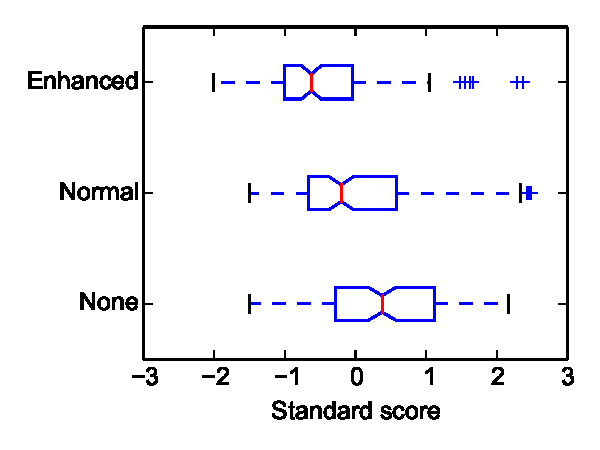
\includegraphics[width=\textwidth]{figs/seek-std.pdf}
  %\caption{Box plot}
  %\label{fig:seekbox}
%\end{subfigure}%
%\begin{subfigure}{.5\textwidth}
  %\centering
  %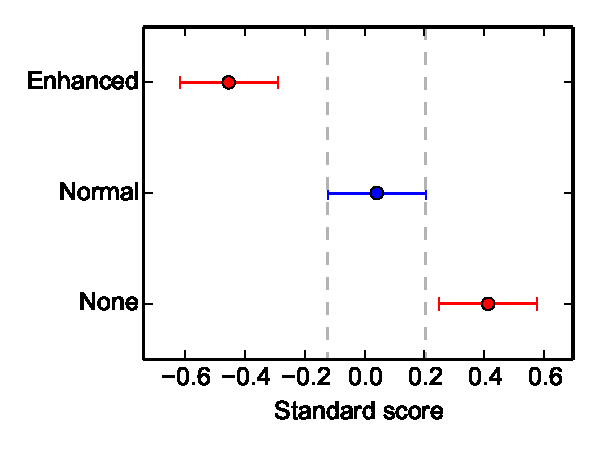
\includegraphics[width=\linewidth]{figs/seek-std-tukey99.pdf}
  %\caption{Tukey's test (99\% confidence interval)}
  %\label{fig:seektukey}
%\end{subfigure}
%\caption{Number of seek actions, standardised per participant}
%\label{fig:seek}
%\end{figure}

\paragraph{Selection time}
The time taken to make a selection was calculated as the difference between the time the play button was first pressed
and the time the final selection was made. This reduces variation due to participants not starting the task immediately
and participants who made a selection, then checked the rest of the recording for other pieces of music. The mean and
standard deviation of the selection time was standardised for each participant to reduce the effect of people's natural
pace.

%\begin{figure}[ht]
%\centering
%\begin{subfigure}{.5\textwidth}
  %\centering
  %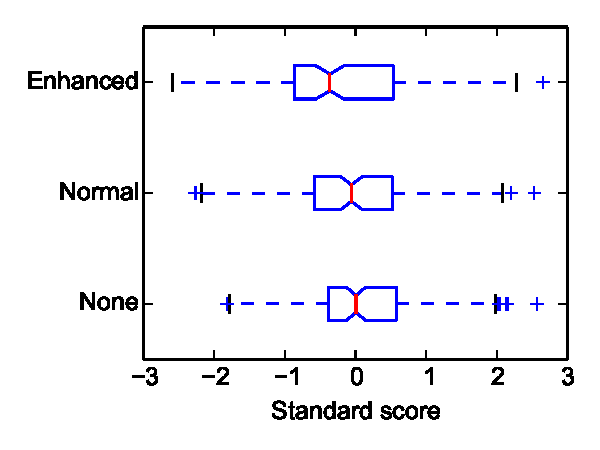
\includegraphics[width=\textwidth]{figs/playstart-to-selectend-std.pdf}
  %\caption{Box plot}
  %\label{fig:selecttimebox}
%\end{subfigure}%
%\begin{subfigure}{.5\textwidth}
  %\centering
  %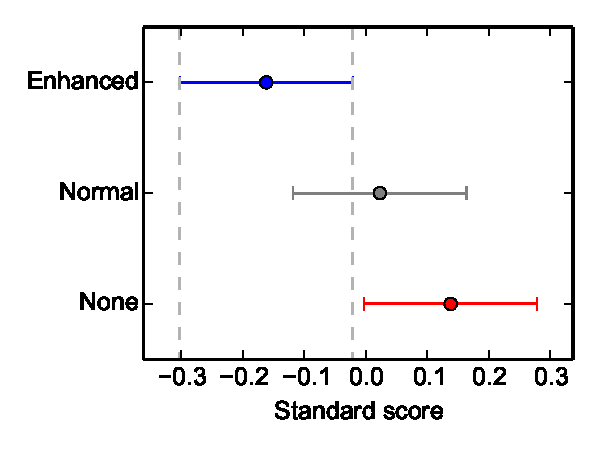
\includegraphics[width=\linewidth]{figs/playstart-to-selectend-std-tukey95.pdf}
  %\caption{Tukey's test (95\% confidence interval)}
  %\label{fig:selecttimetukey}
%\end{subfigure}
%\caption{Selection time (time between start of playback and final selection), standardised per participant}
%\label{fig:selecttime}
%\end{figure}

ANOVA showed that there was a significant difference between visualizations for $p < 0.05$. Tukey's test (see
Figure~\ref{fig:selecttimetukey}) found that there was a difference between no visualization and the colourised version,
but not between either of them and the normal waveform.

\paragraph{Error}
The absolute error of the selections made by each participant were calculated for the inpoint, outpoint and sum of
both. ANOVA found there to be no difference between the visualisations for the inpoint or the sum, but found a
significant difference ($p < 0.05$) for the outpoint.  Tukey's test (see Figure~\ref{fig:outpointerrtukey}) found that
the absolute error of the outpoint for the colourised visualization was significantly lower than the other two
visualizations, but that the other two were no different.

This is an unexpected result which is difficult to explain, as the inpoint and sum errors were not even close to
rejecting the null hypothesis ($p > 0.3$).  Although the result is significant, the improvement in accuracy is only
about 150ms which is small in the context of 5-minute recordings.

%\begin{figure}[ht]
%\centering
%\begin{subfigure}{.5\textwidth}
  %\centering
  %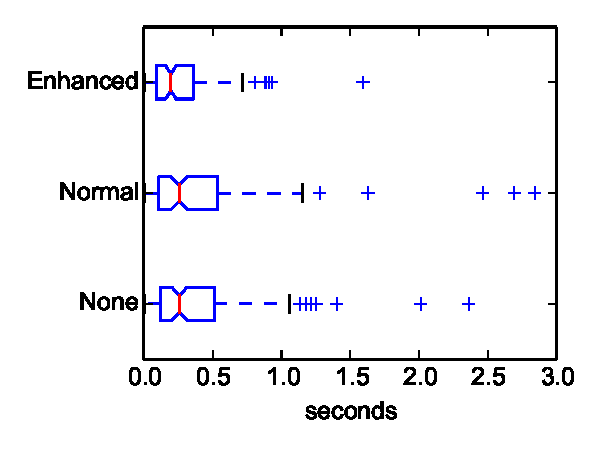
\includegraphics[width=\textwidth]{figs/outpoint-abserr.pdf}
  %\caption{Box plot}
  %\label{fig:outpointerrbox}
%\end{subfigure}%
%\begin{subfigure}{.5\textwidth}
  %\centering
  %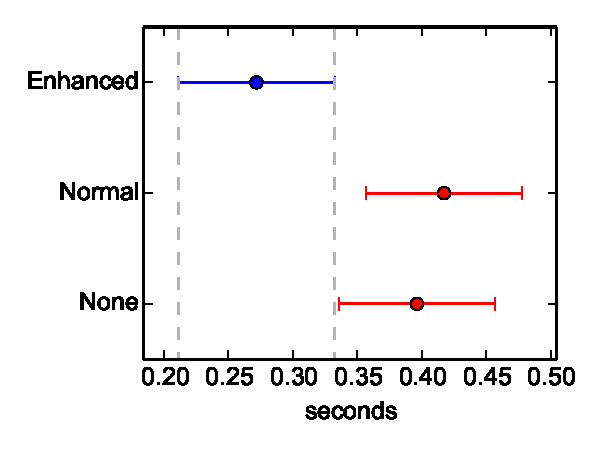
\includegraphics[width=\linewidth]{figs/outpoint-abserr-tukey95.pdf}
  %\caption{Tukey's test (95\% confidence interval)}
  %\label{fig:outpointerrtukey}
%\end{subfigure}
%\caption{Absolute error for the outpoint of selections}
%\label{fig:outpointerr}
%\end{figure}

%\paragraph{Zoom}
%The experimental interface included two displays -- one overview display covering the length of the recording, and a
%zoomed display which showed a magnified part of that. The number of times the zoom in and zoom out buttons were pressed
%was logged. The sum of these values for each visualization is shown in Figure~\ref{fig:zoomtotal}. By subtracting zoom
%out from zoom in, we can infer what the final zoom level was when the response was submitted. The final zoom levels for
%each visualization are shown in Figure~\ref{fig:zoomfinal}.

%\begin{figure}[h!]
%\centering
%\begin{subfigure}{.5\textwidth}
  %\centering
  %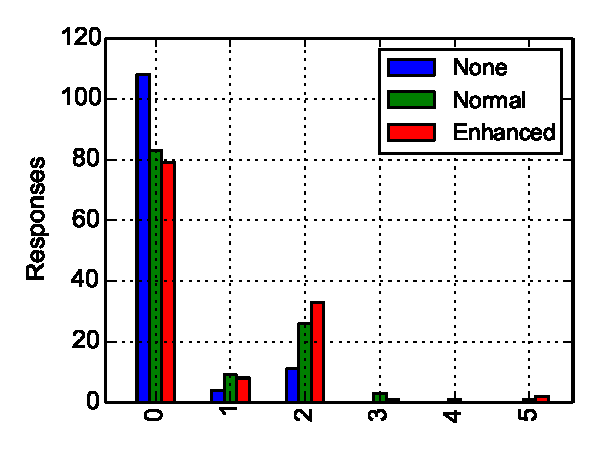
\includegraphics[width=\linewidth]{figs/zoomtotal.pdf}
  %\caption{Total zoom actions}
  %\label{fig:zoomtotal}
%\end{subfigure}%
%\begin{subfigure}{.5\textwidth}
  %\centering
  %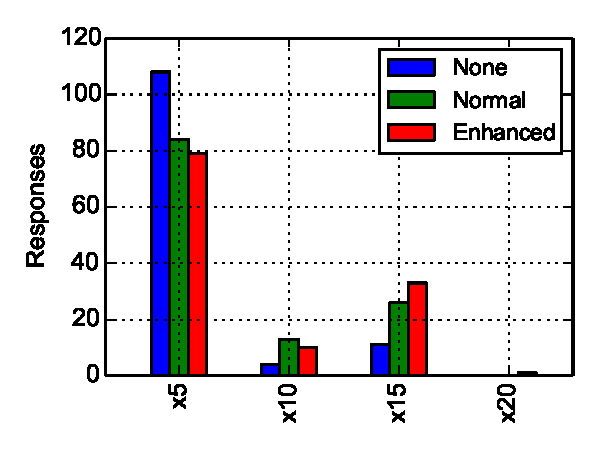
\includegraphics[width=\linewidth]{figs/zoomfinal.pdf}
  %\caption{Final zoom level}
  %\label{fig:zoomfinal}
%\end{subfigure}
%\caption{Analysis of zoom usage}
%\label{fig:zoom}
%\end{figure}

%Most of the time, participants didn't touch the zoom controls and opted to leave it on the default x5 zoom level, which
%displays roughly one minute of audio across 1045 pixels ($\sim$50ms per pixel). Other than the x5 level, x15 was more
%popular than x10 for all visualizations and x20 was barely used at all.

\subsection{Comparison}
Participants were asked to directly compare the three visualizations at the end of the experiment. The results are
shown in Figure~\ref{fig:compare}.

\begin{figure}[ht]
\centering
\begin{subfigure}{.5\textwidth}
  \centering
  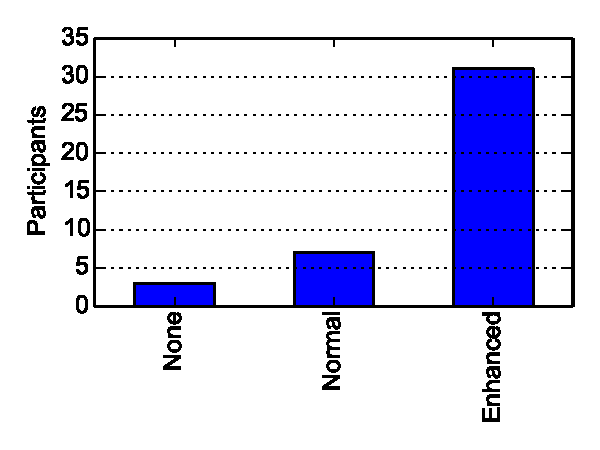
\includegraphics[width=\textwidth]{figs/easiest.pdf}
  \caption{Easiest to use}
  \label{fig:easiest}
\end{subfigure}%
\begin{subfigure}{.5\textwidth}
  \centering
  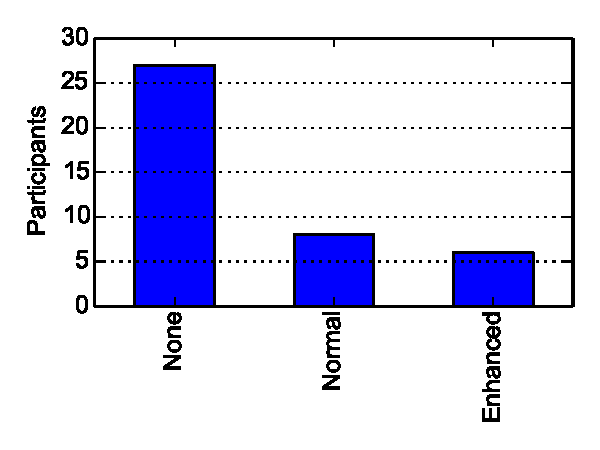
\includegraphics[width=\linewidth]{figs/frustrating.pdf}
  \caption{Most frustrating}
  \label{fig:frustrating}
\end{subfigure}
\caption{Response of participants when asked to compare the visualisations
  using different criteria}
\label{fig:compare}
\end{figure}

76\% of participants thought that the colourised waveform was the easiest to use, with the normal waveform receiving
17\% of votes and 7\% for no waveform.  The strong preference for the colourised waveform over the others shows that
participants thought the additional information added using colour made their task easier.

Having no waveform was considered by two-thirds of participants to be the most frustrating condition, followed by the
normal waveform at 20\% and colourised waveform at 15\%. Although this is another strong result in favour of using
waveforms, the results are not quite as strong as the ones on ease of use. It is possible that the false positives and
negatives present in the colourised waveform caused some people to select it as the most frustrating.

\subsection{Task load index}
The TLX responses were standardised to account for variation in the way different people assign scores. The
distributions of the standardised scores for each visualization are shown in Figure~\ref{fig:tlx}.

\begin{figure}
  \centering
  \begin{subfigure}[t]{0.5\textwidth}
    \centering
    \begin{tikzpicture} 
    \begin{axis}[
      width=\textwidth,
      ylabel=Effort,
      xtick={1,2,3},
      xticklabels={Audio,Waveform,Coloured}]
      \addplot[black,mark=*]
        plot[error bars/.cd, y dir=both, y explicit]
        coordinates {
          (1, -0.122) +- (1.49,1.49)
          (2, -2.244) +- (1.51,1.51)
          (3, -4.220) +- (1.28,1.28)
        };
    \end{axis} 
    \end{tikzpicture}
    \caption{Effort}
  \end{subfigure}%
  ~
  \begin{subfigure}[t]{0.5\textwidth}
    \centering
    \begin{tikzpicture} 
    \begin{axis}[
      width=\textwidth,
      ylabel=Frustration,
      xtick={1,2,3},
      xticklabels={Audio,Waveform,Coloured}]
      \addplot[black,mark=*]
        plot[error bars/.cd, y dir=both, y explicit]
        coordinates {
          (1, -0.829) +- (2.03,2.03)
          (2, -2.976) +- (1.67,1.67)
          (3, -5.268) +- (1.24,1.24)
        };
    \end{axis} 
    \end{tikzpicture}
    \caption{Frustration}
  \end{subfigure}%

  \begin{subfigure}[t]{0.5\textwidth}
    \centering
    \begin{tikzpicture} 
    \begin{axis}[
      width=\textwidth,
      ylabel=Mental demand,
      xtick={1,2,3},
      xticklabels={Audio,Waveform,Coloured}]
      \addplot[black,mark=*]
        plot[error bars/.cd, y dir=both, y explicit]
        coordinates {
          (1, -1.390) +- (1.68,1.68)
          (2, -2.585) +- (1.45,1.45)
          (3, -4.585) +- (1.23,1.23)
        };
    \end{axis} 
    \end{tikzpicture}
    \caption{Mental demand}
  \end{subfigure}%
  ~
  \begin{subfigure}[t]{0.5\textwidth}
    \centering
    \begin{tikzpicture} 
    \begin{axis}[
      width=\textwidth,
      ylabel=Performance,
      xtick={1,2,3},
      xticklabels={Audio,Waveform,Coloured}]
      \addplot[black,mark=*]
        plot[error bars/.cd, y dir=both, y explicit]
        coordinates {
          (1, -5.415) +- (1.10,1.10)
          (2, -6.317) +- (1.11,1.11)
          (3, -7.341) +- (0.88,0.88)
        };
    \end{axis} 
    \end{tikzpicture}
    \caption{Performance}
  \end{subfigure}%

  \begin{subfigure}[t]{0.5\textwidth}
    \centering
    \begin{tikzpicture} 
    \begin{axis}[
      width=\textwidth,
      ylabel=Physical demand,
      xtick={1,2,3},
      xticklabels={Audio,Waveform,Coloured}]
      \addplot[black,mark=*]
        plot[error bars/.cd, y dir=both, y explicit]
        coordinates {
          (1, -3.122) +- (1.81,1.81)
          (2, -4.098) +- (1.45,1.45)
          (3, -6.171) +- (1.08,1.08)
        };
    \end{axis} 
    \end{tikzpicture}
    \caption{Physical demand}
  \end{subfigure}%
  ~
  \begin{subfigure}[t]{0.5\textwidth}
    \centering
    \begin{tikzpicture} 
    \begin{axis}[
      width=\textwidth,
      ylabel=Temporal demand,
      xtick={1,2,3},
      xticklabels={Audio,Waveform,Coloured}]
      \addplot[black,mark=*]
        plot[error bars/.cd, y dir=both, y explicit]
        coordinates {
          (1, -3.171) +- (1.75,1.75)
          (2, -3.268) +- (1.51,1.51)
          (3, -4.878) +- (1.39,1.39)
        };
    \end{axis} 
    \end{tikzpicture}
    \caption{Temporal demand}
  \end{subfigure}%
  \caption{Mean TLX values with 95\% confidence intervals}
\end{figure}

\definecolor{lightred}{RGB}{255,204,204}
\definecolor{lightamber}{RGB}{255,204,153}
\definecolor{lightgreen}{RGB}{204,255,204}
\newcommand{\highsig}{\cellcolor{lightgreen}}
\newcommand{\medsig}{\cellcolor{lightamber}}
\newcommand{\nosig}{\cellcolor{lightred}}
\begin{table}
\resizebox{\textwidth}{!}{
\begin{tabular}{ | l | l | l | l | }
\hline
  & Audio vs Waveform & Audio vs Coloured & Waveform vs Coloured \\ \hline
	Seek actions & \highsig$<0.01$ & \highsig$<0.01$ & \highsig$<0.01$ \\ \hline
	Error & \nosig$>0.05$ & \highsig$<0.01$ & \medsig$<0.05$ \\ \hline
	Time & \nosig$>0.05$ & \highsig$<0.01$ & \highsig$<0.01$ \\ \hline
	TLX Effort & \medsig$<0.05$ & \highsig$<0.01$ & \highsig$<0.01$ \\ \hline
	TLX Frustration & \medsig$<0.05$ & \highsig$<0.01$ & \medsig$<0.05$ \\ \hline
	TLX Mental & \nosig$>0.05$ & \highsig$<0.01$ & \highsig$<0.01$ \\ \hline
	TLX Performance & \nosig$>0.05$ & \highsig$<0.01$ & \medsig$<0.05$ \\ \hline
	TLX Physical & \nosig$>0.05$ & \highsig$<0.01$ & \highsig$<0.01$ \\ \hline
  TLX Temporal & \nosig$>0.05$ & \nosig$>0.05$ & \medsig$<0.05$ \\ \hline
\end{tabular}}
\caption{$p$-values of pairwise comparisons}
\end{table}

%\begin{figure}[p]
  %\centering
  %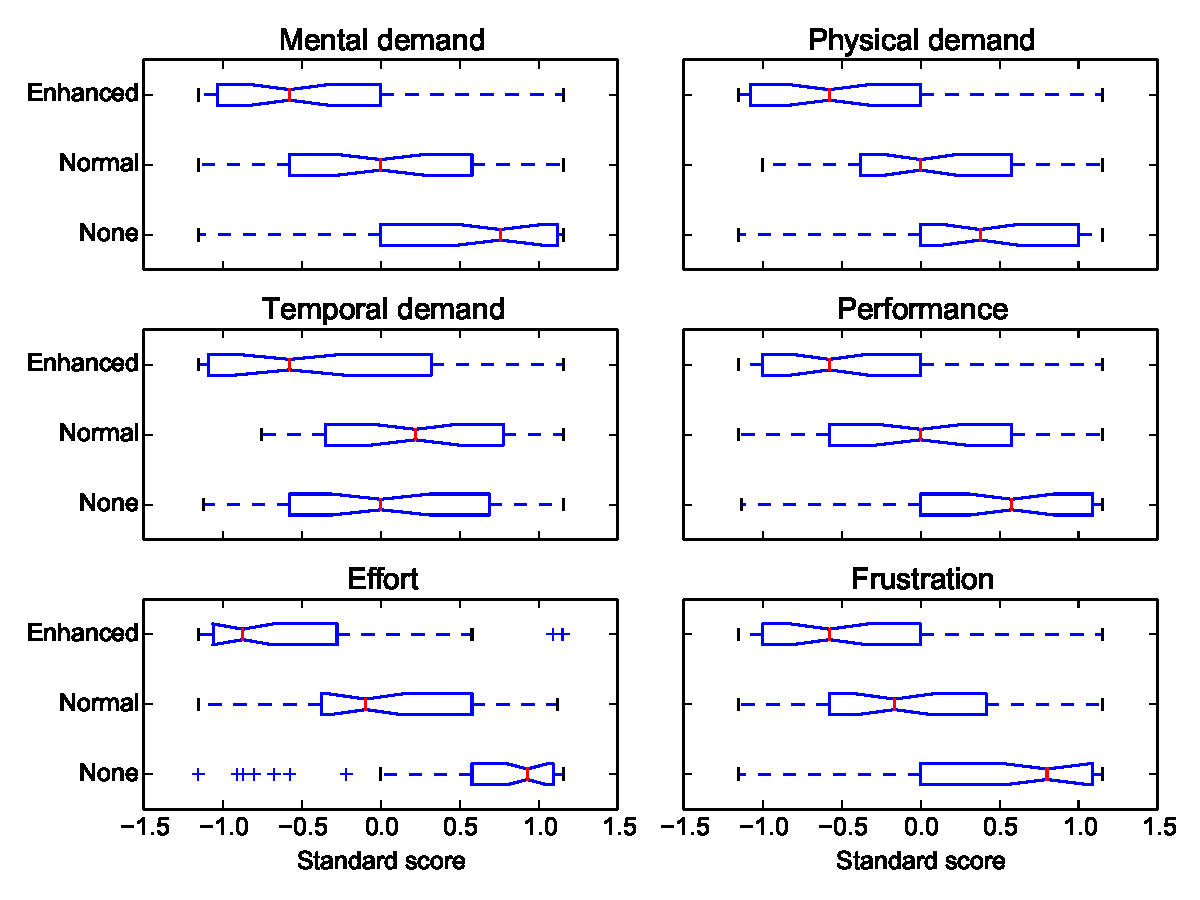
\includegraphics[width=\textwidth]{figs/tlx-std.pdf}
  %\caption{Standard score of NASA Task Load Index responses for each visualization, standardised per participant.}
  %\label{fig:tlx}
%\end{figure}

%\begin{figure}[p]
  %\centering
  %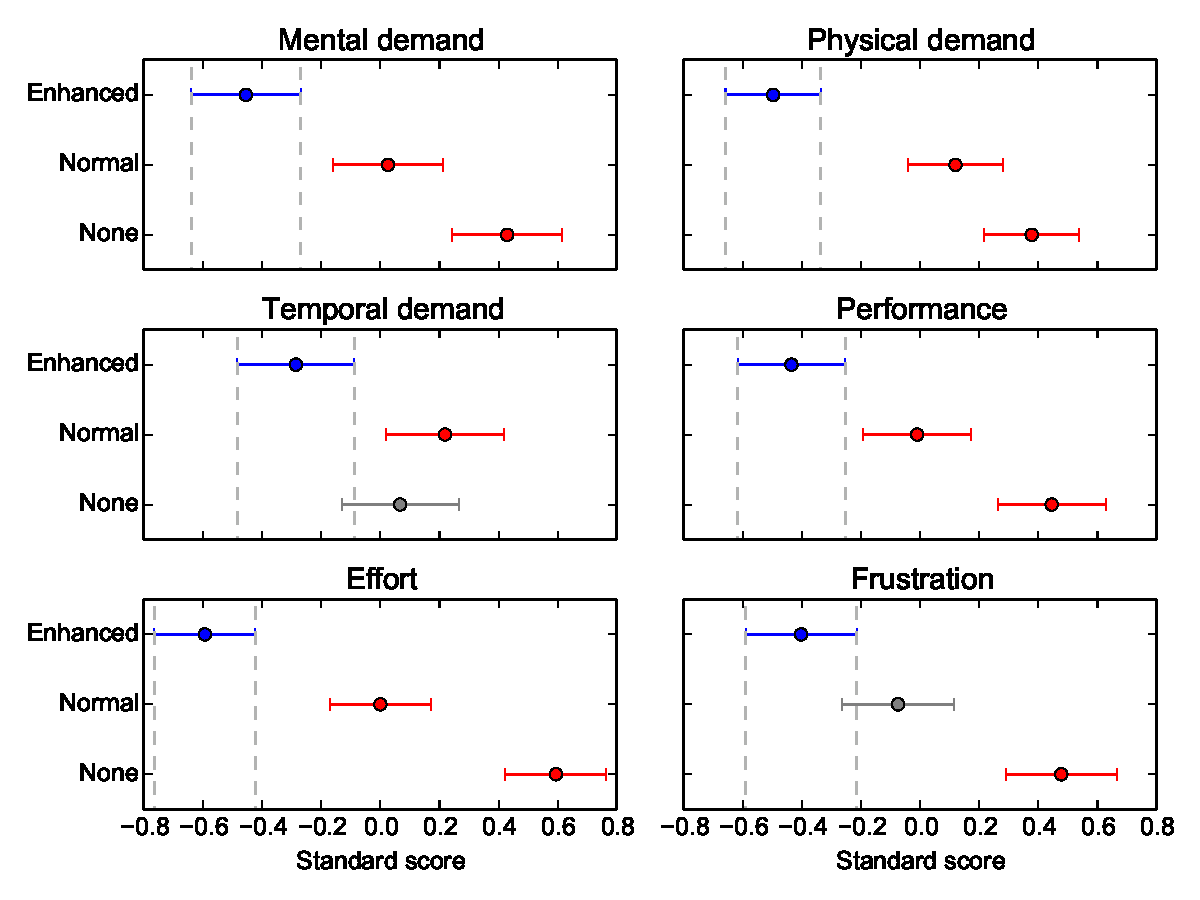
\includegraphics[width=\textwidth]{figs/tlx-std-tukey95.pdf}
  %\caption{Standard score of NASA Task Load Index responses for each visualization, standardised per participant.}
  %\label{fig:tlxtukey}
%\end{figure}

ANOVA found there to be significant differences between the visualizations in all TLX metrics for $p < 0.01$. Tukey's
test (see Figure~\ref{fig:tlxtukey}) found that for $p < 0.05$, the colourised waveform outperformed no waveform in all
metrics except temporal demand, and outperformed the normal waveform in all metrics except frustration. The normal
waveform outperformed no waveform in mental demand, performance, effort and frustration.

Some scepticism should be given to the physical and temporal demand metrics, as it's not entirely clear what is meant
by that terminology in the context of the task. Participants are not working against the clock, not are they doing
anything other than moving the mouse. Although some participants may consider fewer clicks of the mouse to represent
reduced physical demand, we cannot assume that others thought the same.

\subsection{Interaction behaviour}
This section looks at how participants used the features available in the online audio interface, full described in
Section~\ref{sec:iface}.
%Informal observation of some participants as they completed the experiment
%revealed that some people used the interface in different ways. For example,
%when one participant had completed their selection, they scanned through the
%remaining unselected content to check that there were no other pieces of music.

%\begin{figure}[ht]
%\centering
%\begin{subfigure}{.5\textwidth}
  %\centering
  %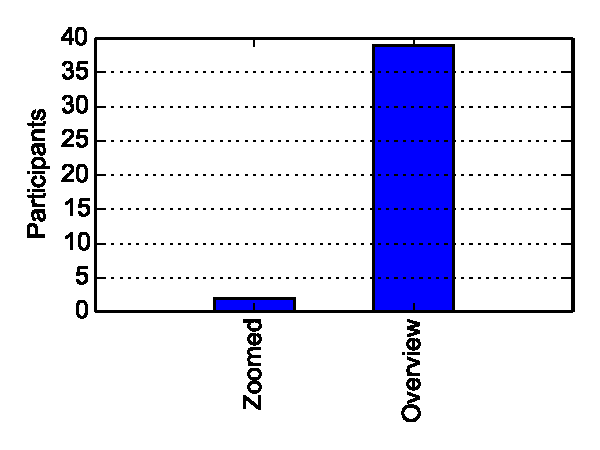
\includegraphics[width=\linewidth]{figs/top-v-bot-pref.pdf}
  %\caption{Display}
  %\label{fig:displaypref}
%\end{subfigure}%
%\begin{subfigure}{.5\textwidth}
  %\centering
  %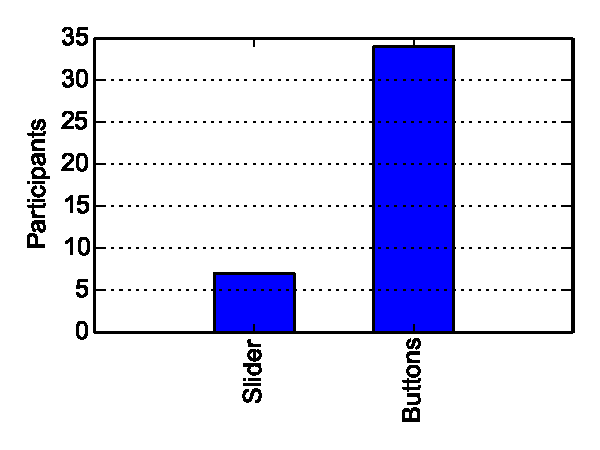
\includegraphics[width=\linewidth]{figs/mark-v-slide-pref.pdf}
  %\caption{Selection method}
  %\label{fig:selectpref}
%\end{subfigure}
%\caption{Preference of participants}
%\label{fig:pref}
%\end{figure}

%\paragraph{Top/bottom display}
%There are two displays that make up the interface -- a zoomed display at the top and an overview display on the bottom.
%Either of the displays can be used to navigate the recording and make selections.

%For each participant, the number of tasks where they used the zoom display more than the overview (and vice-versa) were
%counted. Figure~\ref{fig:displaypref} shows number of participants who, on average, used the zoomed or overview display
%more.

%The results show a clear preference for using the overview display more than the zoom display. Coupled with the results
%of zoom usage in Section~\ref{sec:studymetrics}, we can see that for this task most people opted just to work in the
%overview display, despite only having a resolution of roughly 300ms per pixel.

%An analysis of the overview and zoom display's usage between different visualization methods did not find any notable
%difference.

%\paragraph{Selection method}
%The design of the interface gave participants two methods of making a selection -- buttons to mark in and out points
%using the cursor, and a slider where the in and out points could be dragged around. The cursor can be moved around in
%both the overview and zoomed displays, whereas the slider is only available at the x1 zoom level. This makes the
%buttons more useful for fine edits, where high precision is needed. When using the slider, the selection display
%updates as you move it making it easier for people to see where their selection is.

%For each response, the method with the most actions was found and these preferences were summed for each participant to
%calculate their overall preference. The results are shown in Figure~\ref{fig:selectpref}.

%The buttons were the most popular method of making a selection, with only 17\% of people using the slider more.
%Informal feedback found that some people has a strong preference for using the slider but were frustrated that there
%wasn't a second slider available on the zoomed display.

%\section{Results}
%63 responses were received in the three weeks the experiment ran. 35\% of participants were rejected, which was higher
%than expected. An analysis of the rejected participants found that none had experience of using professional audio
%editing software, which suggests that the errors could be due to lack of experience with audio interfaces.

%The demographic of accepted participants reflected the population which was recruited: 80\% male with a larger
%proportion in the 26-45 age range. This imbalance is not expected to affect the result. Two-thirds of accepted
%participants had experience of using professional audio editing software, with the remaining participants having
%consumer-level experience or less. 39\% reported having no professional experience with audio.

%Figure~\ref{fig:seekpdf} shows the distribution of the number of seek actions for each visualization. On average, the
%number of seek actions required to select the music is lowest for the enhanced waveform and highest for no waveform.
%However, individual participants had different styles of interaction; for example, some people had a tendency to seek
%around a lot whereas others didn't. In order to account for this, the performance and TLX metrics were standardised for
%each participant.

%\begin{figure}[!h]
%\centering
%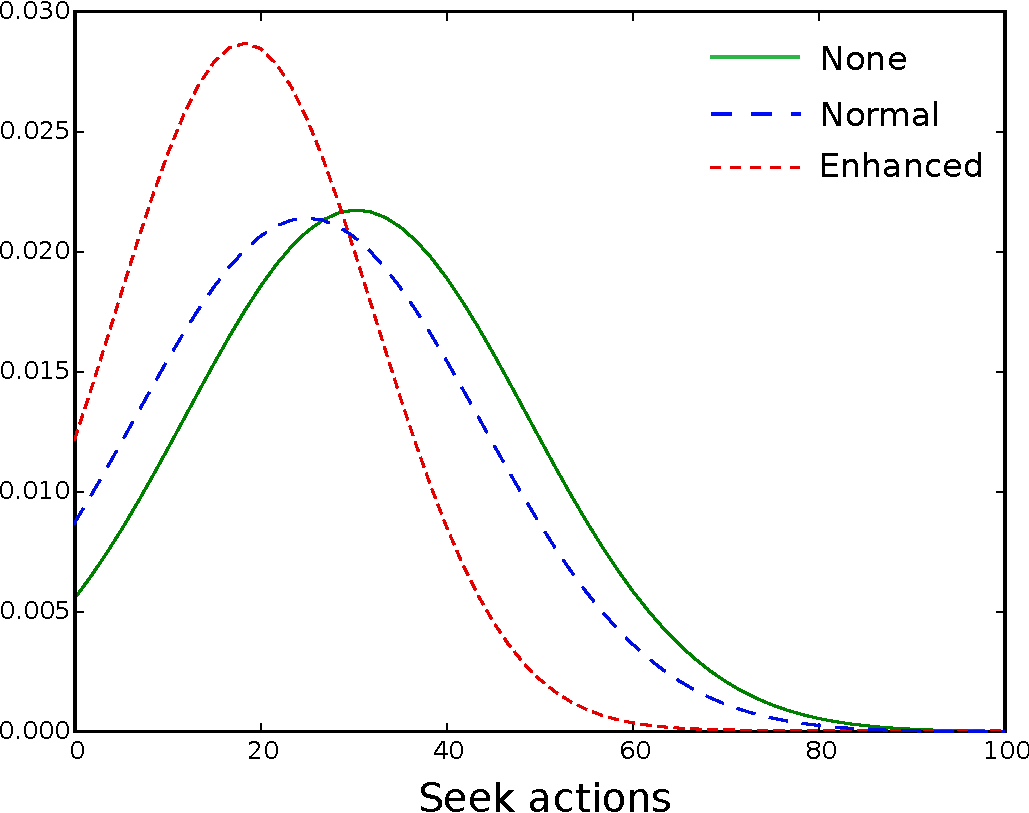
\includegraphics[width=0.6\columnwidth]{figs/seek-pdf.pdf}
%\caption{Probability density function of number of seek actions for each
%visualization}
%\label{fig:seekpdf}
%\end{figure}

%For each metric, the standardisation function (see Equation~\ref{eq:standard}) subtracts the mean of the participant's
%scores and divides by the standard deviation. This maps observations to the `standard score', which is a dimensionless
%unit that represents the number of standard deviations an observation is above the mean.

%\begin{equation}
%std(x) = \frac{x - \mu_{part}}{\highsigma_{part}}
%\label{eq:standard}
%\end{equation}

%The performance and TLX metrics of the 41 accepted participants were analysed using ANOVA.  Significant results were
%found for the number of seek actions ($F_{2,40}=30, p<0.001$) and the selection time ($F_{2,40}=3.2,p\medsig$<0.05$$).  Tukey's
%test shows that the enhanced waveform required fewer seek actions than the normal waveform, and the normal waveform
%required fewer than no waveform (see Figure~\ref{fig:tukeyseekselect}). The selection time was shorter for the enhanced
%waveform compared to no waveform, but the normal waveform was not significantly different.

%\begin{figure}[!h]
%\centering
%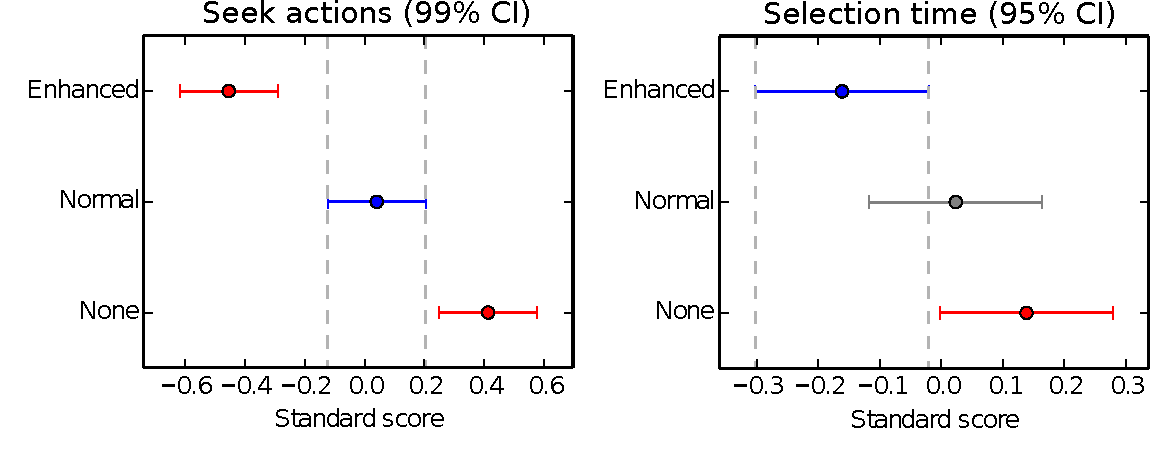
\includegraphics[width=\columnwidth]{figs/seek-select.pdf}
%\caption{Tukey's test for mean number of seek actions and mean selection time}
%\label{fig:tukeyseekselect}
%\end{figure}

%Significant results were found for each of the NASA-TLX metrics ($F_{2,40}>4.8,p\highsig$<0.01$$). The normal waveform performed
%better than no waveform for mental demand, performance, effort and frustration (see Figure~\ref{fig:tlx}). The enhanced
%waveform performed better than the normal waveform for mental, physical and temporal demand, performance and effort.

%\begin{figure}[!h]
%\centering
%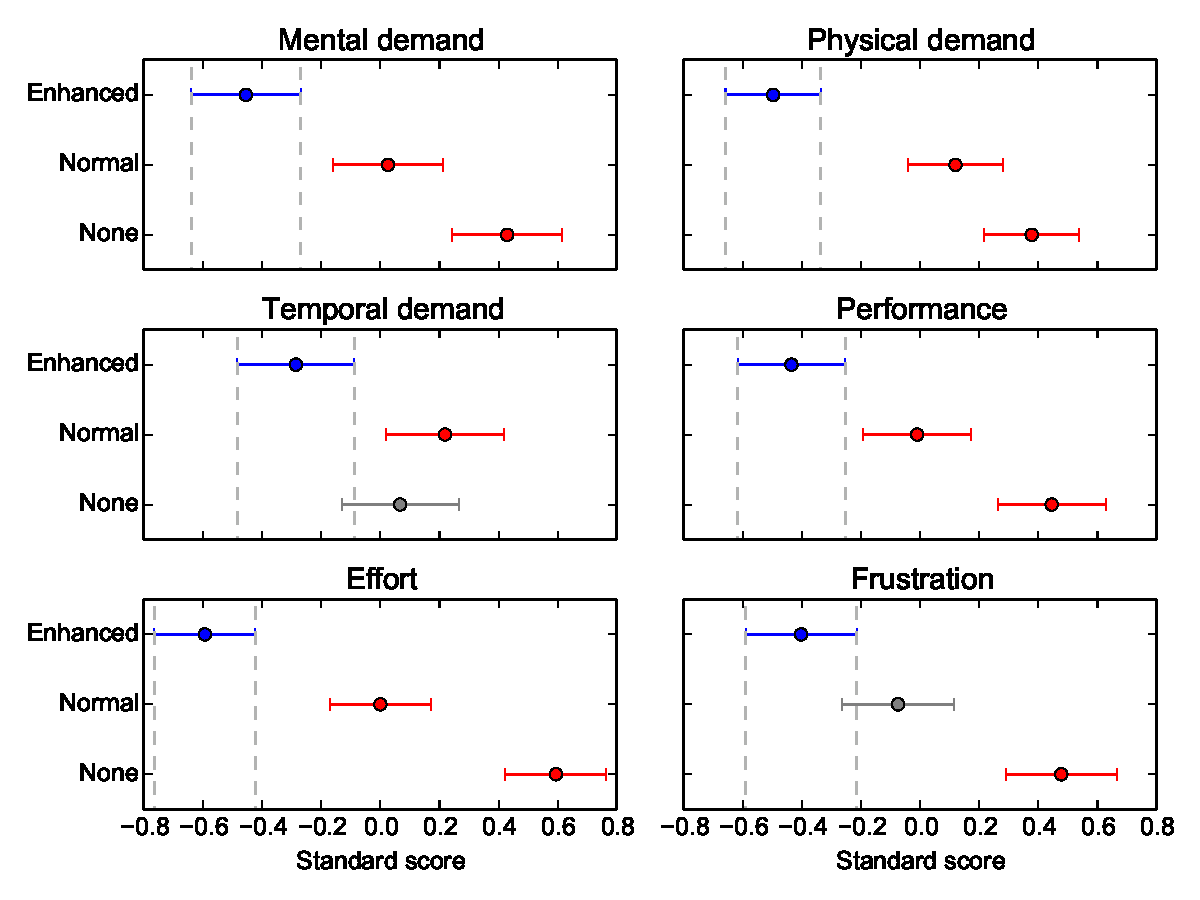
\includegraphics[width=\columnwidth]{figs/tlx-std-tukey95.pdf}
%\caption{Tukey's test for mean of NASA-TLX metrics (95\% CI). Lower is
  %better.}
%\label{fig:tlx}
%\end{figure}

%76\% of participants thought that the enhanced waveform was the easiest to use with the normal waveform scoring 17\%.
%Two-thirds thought that having no waveform was the most frustrating condition with 20\% choosing the normal waveform.

\section{Discussion}

\section{Conclusion}
The normal waveform required fewer seek actions than nothing but was not significantly faster. It scored better than
nothing for mental demand, performance and frustration.

The enhanced waveform required fewer seek actions than the normal waveform and was significantly faster than nothing.
It performed better than the normal waveform for mental demand, performance and effort.

%This experiment used a browser-based audio interface to conduct a within-subjects online study of how users performed
%in finding and selecting music with different audio waveforms. Three conditions were tested -- no waveform, a normal
%waveform and a waveform that was colourised using a simple speech/music discriminator.

%Compared to no waveform, the normal waveform required fewer seek actions and was rated better in terms of mental
%demand, performance, effort and frustration. Finding and selecting music with the colourised version took less time
%than with no waveform. Compared to the normal waveform, it required fewer seek actions and was rated better in terms of
%mental, physical and temporal demand, performance and effort.

%\subsection{Further work}
%The results indicate that the waveform can be significantly improved, even with a simple enhancement. The next stages
%of this research will focus on development of audio analysis and visualization algorithms/tools that address the needs
%of people working in radio production. This will be followed by an analysis of the real-world benefit of using these
%new tools.
